%Para este capítulo se usará la abreviatura "const".
\chapter{Construcciones de espacios}
\label{const}
%Introducción por hacer.
\section{Imágenes inversas (inmersiones)}
\subsection{Construcción de continuidad menos fina}
Esta sección se centrará en dar solución al siguiente problema. Dado un espacio topológico $(\mathcal{X},\T)$, un conjunto $\mathcal{Y}$ y una aplicación $f$ que nace en $\mathcal{Y}$ y muere en $(\mathcal{X},\T)$, queremos dotar a $\mathcal{Y}$ de una topología que haga que $f$ sea continua.

Visto en forma de diagrama
\begin{equation*}
\xymatrix{
	(\mc{Y},\T_y) \ar[r]^f
	&(\mathcal{X},\T)}
\end{equation*}

\begin{obs}[Solución trivial]
	Evidentemente, una elección fácil para que esto ocurra es escoger la topología discreta, puesto que es la que cuenta con más abiertos y, por lo tanto, para todo abierto $\U'$ de $\mathcal{X}$ entonces $f^{-1}(\U')$ es abierto en $\mathcal{Y}$, lo que implica que $f$ es continua.
\end{obs}
Sin embargo, este caso no es realmente interesante, por lo cual refinaremos el enunciado de nuestro problema, ahora no buscaremos una topología cualquiera sino la topología menos fina posible que haga continua a $f$.
\begin{obs}[Aproximación a la solución]
	Un truco que se nos podría ocurrir para atacar este problema es usar la caracterización de la continuidad que afirma que una aplicación $f$ es continua si y solo si transforma abiertos en abiertos por imágenes inversas.
	
	Usando esto, es claro que la topología que buscamos deberá tener como abiertos al menos a las imágenes inversas de los abiertos de $\X$. De hecho, como vemos ahora mismo, esta es la solución de nuestro problema.
\end{obs}
La solución a este problema es la topología $f^{-1}(\T)$, definida como 
\[f^{-1}(\T):=\{f^{-1}(\U)\midc\U\in \T\}\]
y que llamamos \tbitop{imagen inversa}.

La comprobación de que verdaderamente es una topología se desprende de las propiedades de la función inversa aplicada a conjuntos. Por otro lado, es la menos fina que hace a $f$ continua por construcción, luego cualquier otra topología con estas características contiene a esta. Finalmente, se tiene que es única. En efecto, si tenemos que $\T$ y $\T'$ cumplen que son las menos finas por construcción, entonces se tiene que $\T\subset \T'$ y $\T'\subset \T$, luego son iguales.

\subsection{Caracterización de la continuidad entrante}
Es hora de profundizar un poco más. Tomemos otro espacio topológico arbitrario $(Z,\T')$ y consideremos una función $g$ que nace en este y muere en $\Y$.

El problema que se nos plantea ahora es determinar qué aplicaciones $g:Z\to \Y$ son continuas.

Damos sin rodeos la solución a este problema.
\begin{prop}[Propiedad universal de las inmersiones]
	\label{const_universalInmersiones}
	Una aplicación $g:Z\to\Y$ es continua si y solo si se verifica que $f\circ g$ es continua.
\end{prop}
\begin{proof}
	Para ponernos en situación nos dibujamos el diagrama
	\begin{equation*}
	\xymatrix{
		&(\Y,f^{-1}(\T)) \ar[r]^f
		&(\X,\T) \\
		&(Z,\T') \ar@{-->}[ru]_{f\circ g} \ar[u]^g}
	\end{equation*}
	En primer lugar, observemos que como $f$ es continua por definición, si $g$ es continua, entonces trivialmente la composición $f\circ g$ también lo será. Con lo que la primera de las implicaciones es evidente.
	
	Recíprocamente, queremos ver que $g$ transforma abiertos en abiertos por imágenes inversas. En efecto, dado $W\in f^{-1}(\T)$, comprobemos que $g^{-1}(W)\in\T'$. Por definición $W=f^{-1}(\U)$, con $\U\in\T$. Por ende,
	\begin{equation*}
		g^{-1}(W)=g^{-1}(f^{-1}(\U))=(f\circ g)^{-1}(\U)
	\end{equation*}
	Como $f\circ g$ es continua, el resultado se sigue.
\end{proof}
\begin{obs}[Irrelevancia de la topología de $\Y$]
	La proposición \ref{const_universalInmersiones} es realmente interesante, puesto que nos dice que la topología que haya en $\Y$ no es relevante a la hora de estudiar las aplicaciones continuas que mueren en $\Y$.
\end{obs}
\subsection{Propiedad universal de las inmersiones}
\begin{defi}[Propiedad universal]
	Si para cierta topología $\T_\Y$ de $\Y$ se verifica el enunciado de la proposición \ref{const_universalInmersiones} se dice que la topología $\T_\Y$ verifica la \tbi[propiedad universal!de las inmersiones]{propiedad universal de las inmersiones}.
\end{defi}
Ahora tratamos de determinar para qué topologías de $\Y$ se verifica la propiedad universal para las inmersiones.

Desde luego, la proposición \ref{const_universalInmersiones} nos dice que para la topología $f^{-1}(\T)$ se verifica la propiedad universal (y que es la menos fina que lo hace, pues es la menos fina que hace a $f$ continua).

Ahora vamos a ver que no solo ocurre esto sino que es la única topología que verifica esta propiedad universal.

\begin{prop}[Unicidad de la propiedad universal]
	Sea $\T_\Y$ una topología que verifica la propiedad universal, entonces $\T_\Y=f^{-1}(\T)$.
\end{prop}
\begin{proof}
	Razonaremos por doble contención y haciendo algunos cambalaches útiles para retorcer la propiedad universal a nuestro gusto.
	
	Consideramos el siguiente diagrama, análogo al de la demostración de la proposición \ref{const_universalInmersiones} pero tomando $(Z,\T')=(\Y,\T_\Y)$ y $g=\text{id}$.
	\begin{equation*}
	\xymatrix{
		&(\mathcal{Y},\T_{\mathcal{Y}}) \ar[r]^f
		&(\mathcal{X},\T) \\
		&(\mathcal{Y},\T_{\mathcal{Y}}) \ar@{-->}[ru]_{f\circ \text{id}=f} \ar[u]^{\text{id}}}
	\end{equation*}
	
	Sabemos que la identidad de un espacio en sí mismo es una aplicación continua. De este modo, por la propiedad universal, tenemos por lo anterior que $f\circ\text{id}=f$ es continua. En consecuencia, $\T_{\mathcal{Y}}$ hace que $f$ sea continua y, por tanto, por construcción de $f^{-1}(\T)$, $f^{-1}(\T)\subset \T_\Y$. Ya tenemos demostrada una inclusión.
	
	Para la otra implicación consideramos un diagrama análogo, pero tomando $(Z,\T')=(\Y,f^{-1}(\T))$ y $g=\text{id}$.  
	
	\begin{equation*}
	\xymatrix{
		&(\mathcal{Y},\T_{\mathcal{Y}}) \ar[r]^f
		&(\mathcal{X},\T) \\
		&(\mathcal{Y},f^{-1}(\T)) \ar@{-->}[ru]_{f\circ \text{id}=f} \ar[u]^{\text{id}}}
	\end{equation*}
	
	Ahora, por definición de $f^{-1}(\T)$, sabemos que $f\circ\text{id}=f$ es continua. Ahora, aplicando la propiedad universal tenemos que $\text{id}$ debe ser continua, y esto solo es posible si $\T_\Y\subset f^{-1}(\T)$.
\end{proof}
\begin{obs}[Inyectividad] Vamos a ver ahora un caso particular muy importante (el que realmente es de interés) de esta construcción.

Supongamos que dos puntos $y_1$ e $y_2$ terminan en el mismo punto tras ser evaluados en una aplicación (lo que quiere decir que esta no es inyectiva). Los abiertos $\U$ que contienen a la imagen de los dos puntos mencionados $x$ (que es la misma) cumplen que $f^{-1}(\U)$ contiene a $y_1$ e $y_2$, luego estos dos puntos resultan ser topológicamente indistinguibles (no puedo separarlos en dos abiertos distintos). Por ello, este tipo de aplicaciones no presentan mucho interés puesto que no es posible conocer con certeza ciertas propiedades.
\end{obs}
\subsection{Inmersiones}
El caso verdaderamente interesante ocurre cuando $f$ es inyectiva. En este caso, si se considera el subespacio $(f(\mathcal{\Y}),\left.\T\right|_{f(\mathcal{\Y})}) \subset (\mathcal{\X},\T)$, entonces $f$ es biyectiva:

\[(\mathcal{\Y},f^{-1}(\T)) \xrightarrow{f} (f(\mathcal{\Y}),\left.\T\right|_{f(\mathcal{\Y})}) \subset (\mathcal{\X},\T).\]

Además, la aplicación es \tb{continua} puesto que, dado $\W$ un abierto de $f(\mathcal{\Y})$, entonces, por topología relativa $\W=f(\Y)\cap \U$ para cierto abierto $\U\in \T$. Esto implica que

\[f^{-1}(\W)=f^{-1}(\U\cap f(\mathcal{\Y}))=f^{-1}(\U)\cap \mathcal{\Y}=f^{-1}(\U),\]

que es abierto de $\mathcal{\Y}$ por la definición de topología que hemos tomado.

Sin embargo, esto no termina aquí, ya que $f$ es \tb{abierta}. En efecto, como $\U$ está contenido en $\mathcal{Y}$ e $\mathcal{Y}$ está equipado con la topología inversa de la topología de $\X$, tenemos que existe un abierto $\U \subset \X$ tal que $f^{-1}(\U) = \W$. Aplicando $f$ a esta igualdad obtenemos que $f(\W) = f(f^{-1}(\U)) = \U \cap f(\W)$ que es un abierto de $f(\mathcal{Y})$.

Por tanto, al ser $f$ continua y abierta, es \tb{homeomorfismo}. Esto es sorprendente, ya que una aplicación inyectiva de $\mathcal{\Y}$ en $\mathcal{\X}$ es homeomorfismo de $\mathcal{\Y}$ en $f(\mathcal{\Y})$.

\begin{defi}[Inmersión o embebimiento]
	A una función $f:(\Y,f^{-1}(\T))\to(\X,\T)$ inyectiva se la denomina \tbi{inmersión} o \tbi{embebimiento}.
\end{defi}
\section{Imágenes directas (cocientes e indentificaciones)}

Después de haber realizado todo el desarrollo anterior, una posibilidad que se nos plantea es dualizar las cuestiones que nos han ido apareciendo. Coloquialmente, podríamos decir que vamos a cambiarle el sentido a todo.

Así pues, consideremos un espacio topológico $(\mathcal{\X},\T)$, un conjunto $\mathcal{\Y}$ y una aplicación $f$ que nace en $(\mathcal{\X},\T)$ y muere en $\mathcal{\Y}$. El problema ahora consiste en dotar a $\mathcal{\Y}$ de una topología que haga que $f$ sea continua. La solución más sencilla sería elegir la topología trivial, puesto que sus únicos abiertos son el vacío y el total y siempre se cumpliría que para cada $\U'$ abierto de $\mathcal{\Y}$ entonces la imagen inversa de este es un abierto del espacio de partida. No obstante, es interesante encontrar la topología más fina que cumpla esto, y esta es 

\[f(\T)=\{\U: f^{-1}(\U)\in \T\}\]

Evidentemente, se trata de una topología y es la más fina que permite que $f$ sea continua ya que si se añade algún abierto más deja de serlo. Por último, realizando un razonamiento por doble inclusión al análogo en imágenes inversas, se puede ver que es única. Llamamos a esta topología \tbitop{imagen} o \tb{\ti{topología imagen directa}}.

Continuando con la misma argumentación, veamos cuando una función $g$ que parta de $\mathcal{Y}$ es continua

\begin{equation}
\label{cont_propiedad_universal_top_imagen}
\xymatrix{
	(\mathcal{\X},\T) \ar[r]^f \ar@{-->}[rd]_{g\circ f} &
	\mathcal{\Y} \ar[d]^g & \\
	&(Z,\T')}
\end{equation}

Trabajando igual que en el caso anterior, se llega a que $g$ es continua si y solo si $g\circ f$ es continua (para ello, basta ver que si $\W\subset \T'$ entonces $g^{-1}(\W)\subset f(\T)$) y que $f(\T)$ es la topología en $\mathcal{\Y}$ que cumple esta doble implicación. Decimos que esta es la \tbi[propiedad universal!de la imagen]{propiedad universal de la imagen}.

\begin{obs}[Sobreyectividad]
	
	Supongamos que $f$ no es sobreyectiva y tomemos un punto $y\notin f(\mathcal{\X})$. Entonces $f^{-1}(y)$ es el vacío, pero como el vacío es abierto llegamos a que el punto es abierto, luego $f(\left.\T\right|_{\mathcal{\Y}\backslash f(\mathcal{\X})})$ coincide con la topología discreta. Sin embargo, la imagen inversa de $\mathcal{\Y}\backslash f(\mathcal{\X})$ es vacía y es abierta en la imagen. Además, como $f(\mathcal{\X})$ es el complementario de $\mathcal{\Y}\backslash f(\mathcal{\X})$, entonces $f(\mathcal{\X})$ es cerrado. No obstante, $f(\mathcal{\X})$ coincide con el total, luego también es un abierto. 	
\end{obs}

Ahora que hemos visto que el caso interesante es que $f$ sea sobreyectiva, consideramos el siguiente diagrama:
\[\xymatrix{
	(\X,\T) \ar[r]^{f} \ar[d]_{p} &
	(\mc{Y}, f(\T)) \\
	\X/\mathord{\sim}  \ar[ru]_{\bar{f}}
}\]
donde la relación de equivalencia verifica $x\sim y\iff f(x)=f(y)$. Aquí, $p$ es simplemente la aplicación que manda $x\in\X$ a su clase de equivalencia, y consideramos $\bar{f}$ de forma que verifique que $f=\bar{f}\circ p$.

% Esto no lo nombró él en clase pero lo he encontrado por ahí y es cómodo
Decimos que una aplicación $f$ que verifica que si $x\sim y$ entonces $f(x)=f(y)$ respeta la relación de equivalencia $\mathord{\sim}$. Nótese que no se exige la equivalencia, solo la implicación.

Como hemos definido la relación de equivalencia como la que verifica $x\sim y\iff f(x)=f(y)$, tenemos que $\bar{f}$ es una biyección. Además, se puede comprobar que si existe $\bar{f}$ tal que $f=\bar{f}\circ p$, entonces $f$ respeta la relación de equivalencia $\mathord{\sim}$.

Ahora, vamos a definir la topología cociente para $\X/\mathord{\sim}$. Buscamos una topología que verifique que la aplicación $p$ es continua y que existe una aplicación continua $\bar{f}$ que respete la relación de equivalencia $\mathord{\sim}$ y que verifique que $f=\bar{f}\circ p$.

\begin{defi}[Topología cociente]
	Definimos la \tbitop[$\T/\mathord{\sim}$]{cociente} en las condiciones anteriores como:
	\[\T/\mathord{\sim} = \{V\midc p^{-1}(V)\in\T\}\]
	es decir, la topología cociente es la topología imagen por $p$.
\end{defi}

Está claro que se verifican nuestros requisitos. Por un lado, $p$ es trivialmente continua (pues la topología imagen por $p$ es precisamente la que verifica esto). Por otro lado, por ser una topología imagen se verifica directamente la continuidad de $\bar{f}$.

\begin{prop}
	En las condiciones de la construcción (cuando la relación $\sim$ está definida como $x\sim y\iff f(x)=f(y)$), $\bar{f}$ es homeomorfismo.
	
	\begin{proof}
		Ya hemos visto que $\bar{f}$ es biyectiva cuando la relación de equivalencia verifica $x\sim y\iff f(x)=f(y)$, y que es continua en el sentido en el que la hemos definido. Para ver la continuidad en el otro sentido, basta con ver que $\bar{f}$ es abierta.
		
		En efecto, sea $U\in \X/\mathord{\sim}$ abierto. Tenemos que $p^{-1}(U)=f^{-1}(\bar{f}(\U))$, porque:
		\[x\in p^{-1}(U)\iff p(x)\in \U\stackrel{\bar{f}\text{ biy.}}{\iff}\bar{f}(p(x))\in \bar{f}(U)\iff f(x)\in\bar{f}(U)\iff x\in f^{-1}(\bar{f}(U))\]
		
		Entonces, como $\U$ es abierto y $p$ continua, $p^{-1}(U)$ es abierto, luego $f^{-1}(f(\U))$ también es abierto. Ahora por definición de la topología de $\mathcal{Y}$ tenemos que $\bar{f}(\U)$ es abierto en $\mathcal{Y}$.
		
	\end{proof}
\end{prop}

Por otro lado, está claro que todos los abiertos de $\T/\mathord{\sim}$ son imágenes por $p$ de abiertos de $\T$ (pero no todas las imágenes de abiertos tienen que estar necesariamente en $\T$). Entonces, definimos:

\begin{defi}[Conjunto saturado]
	En las condiciones anteriores, decimos que $W\in\T$ es \tbi[conjunto!saturado]{saturado} si $W=p^{-1}(p(W))$. Es equivalente decir que $[x]\cap W\neq\emptyset\implies [x]\subset W$, o que $x\in W,y\sim x\implies y\in W$.
\end{defi}

Gracias a esta definición, podemos reescribir la topología cociente como:
\[\T/\mathord{\sim} = \{p(W)\midc W\in\T\text{, } W\text{ saturado}\}\]

Además, vamos a dar un nombre a las funciones que envían $X$ en un espacio homeomorfo a un cociente:

\begin{defi}[Identificación]
	Una \tbi{identificación} es una aplicación $f:(X,\T)\to (\mc{Y},\T')$ sobreyectiva que verifica que $\T'$ es la topología imagen por $f$: $f(\T)$.
\end{defi}

La aplicación $f$ con la que hemos estado trabajando es, entonces, una identificación. El hecho de que la topología de $\mc{Y}$ sea la imagen significa que una identificación es continua.

Las identificaciones se llaman a veces en la literatura aplicaciones cociente\index[general]{aplicación!cociente}. Esto está ligado con su utilidad: las identificaciones son aquellas que inducen una relación de equivalencia $\sim$ de forma que podemos desarrollar toda la construcción anterior. De esta forma, nos ``regalan'' un espacio homeomorfo a $\mc{Y}$ que a menudo es más simple y más fácil de entender que él. Este propósito quedará más claro en los ejemplos posteriores.

Para comprobar si una aplicación es una identificación, podemos usar la siguiente proposición:

\begin{prop}[Condiciones suficientes de identificación]
	Sea $f:\X\to\mc{Y}$ una aplicación. Si se verifica alguna de las siguientes condiciones, $f$ es una identificación:
	\begin{enumerate}
		\item $f$ es una aplicación continua abierta.
		\item $f$ es una aplicación continua cerrada.
	\end{enumerate}
\end{prop}

Nótese que puede haber identificaciones que no verifiquen ninguna de las condiciones anteriores. Además, como no se exige que las identificaciones sean biyectivas, las dos condiciones anteriores no son equivalentes.

Toda esta construcción abstracta debe servirnos para formalizar todo el concepto de cociente de un espacio. Esta es quizá la idea más importante que se va a ver en toda la asignatura, y es excepcionalmente útil para construir una gigantesca variedad de homeomorfismos y encontrar objetos simples homeomorfos a otros mucho más complejos.

\begin{exa}[Circunferencia unidad]
	Definimos la aplicación:
	\[\begin{split}
	\R&\to\esfera^1 \\
	t&\mapsto e^{2\pi it}=(\cos 2\pi t,\sen 2\pi t)
	\end{split}\]
	y consideramos la relación de equivalencia $s\sim t\iff e^{2\pi is}=e^{2\pi it}\iff s-t\in\Z$. Vamos a ver que la circunferencia unidad $\esfera^1$ es homeomorfa a $\R/\mathord{\sim}$.
	
	Nos queda, pues, el siguiente esquema:
	\[\xymatrix{
		\R \ar[r] \ar[d] &
		\esfera^1 \\
		\R/\mathord{\sim}  \ar@{<->}[ru]
	}\]
	y está claro que la aplicación que manda $\R$ a $\esfera^1$ es una identificación, pues es sobreyectiva, continua y homeomorfismo local, luego es abierta.
	
	Ahora, nótese que considerando $[0,1]\subset\R$ podemos tomar las restricciones correspondientes con el siguiente esquema:
	\[\xymatrix @C=0.5pc @R=0.5pc @L=-0.2pc {
		& \R \ar[rr] \ar[dd] & &
		\esfera^1 \\
		[0,1] \ar@{}[ur]^*[@]{\subset} \ar[dr] \\
		& \R/\mathord{\sim}  \ar@{<->}[rruu]
	}\]
	y llegar a otra identificación. Ahora la relación de equivalencia asociada es simplemente aquella en la que $1\sim 0$ y todos los demás puntos son solamente equivalentes a sí mismos.
\end{exa}

Esta posibilidad de encontrar, a veces, un cociente más simple que tiene la misma topología nos motiva a definir:

\begin{defi}[Dominio fundamental]
	En una construcción como la anterior, llamamos \tbi{dominio fundamental} a la región cerrada más pequeña posible con un representante de cada clase de equivalencia. Según la situación, a veces se exigen también otras propiedades como compacidad.
\end{defi}

\begin{exa}
	Ahora, vamos a considerar el toro de revolución que vive en $\R^3$, cuya parametrización es conocida:
	\[\begin{split}
	x&=(a\cos(\theta)+b)\cos(\phi),\\
	y&=(a\cos(\theta)+b)\sin(\phi),\\
	z&=a\sin(\theta).
	\end{split}\]
	
	Como vemos en la imagen, se trata de una figura generada por revolución de una circunferencia en torno a un eje.
	
	\begin{figure}[h!]
		\centering
		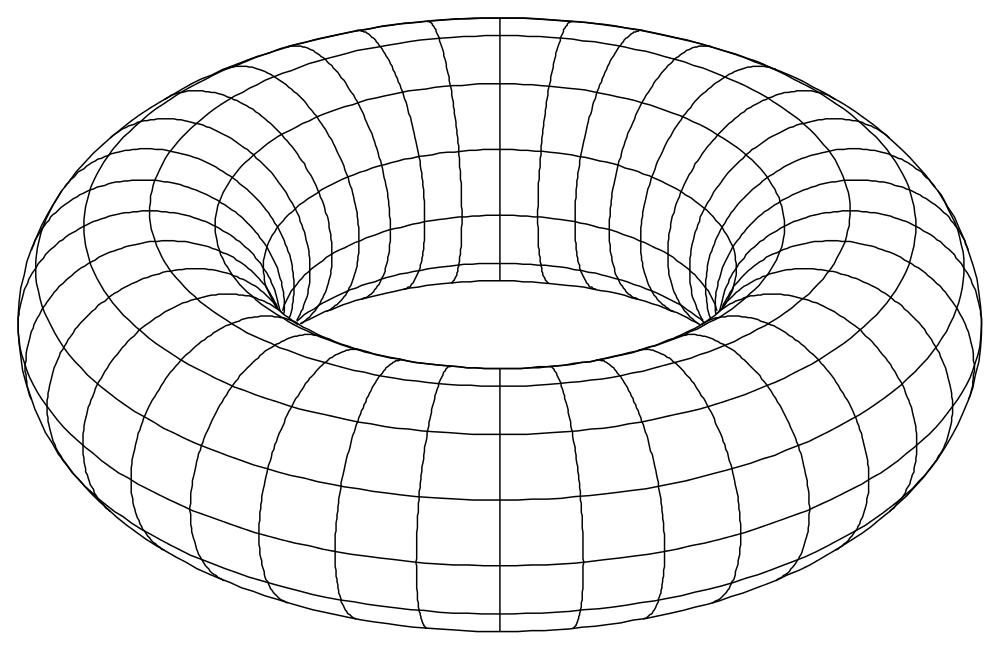
\includegraphics[scale = 0.15]{img/toro}
	\end{figure}
	
	Vamos a hacer pues una construcción similar a la ya vista para la circunferencia unidad. Nos queda un esquema del siguiente tipo:
	
	\[\xymatrix @C=0.5pc @R=0.5pc @L=-0.2pc {
		& \R^2\ar[rr] \ar[dd] & &
		\toro^2\subset\R^3 \\
		[0,2\pi]^2 \ar@{}[ur]^*[@]{\subset} \ar[dr] \\
		& \R^2/\mathord{\sim}  \ar@{<->}[rruu]
	}\]
	
	En este caso, la relación de equivalencia está definida como:
	\[(x,y)\sim (x',y')\iff x-x'\in\Z,\;y-y'\in\Z\]
	y como dominio fundamental encontramos el cuadrado $[0,2\pi]^2$. 
	
	A menudo, los dominios fundamentales se representan con esquemas llamados \tbi[polígono fundamental]{polígonos fundamentales}. La forma de entenderlos es que la relación de equivalencia ``pega'' los puntos de $A$ y de $B$ en el sentido que indican las flechas, como vemos en el ejemplo siguiente, que representa el toro que acabamos de describir:
	
	% Copiado de https://en.wikipedia.org/wiki/Fundamental_polygon . Querría hacer uno yo pero no ha dado tiempo.
	\begin{figure}[h!]
		\centering
		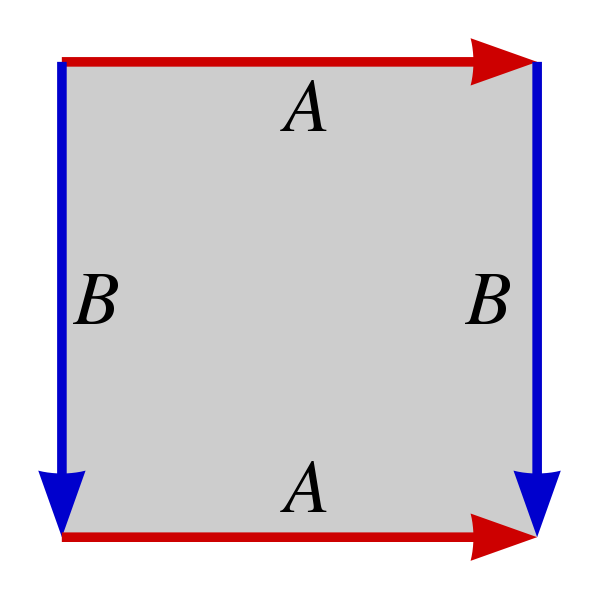
\includegraphics[scale = 0.1]{img/pol_fund_toro}
	\end{figure}
\end{exa}

En el siguiente ejemplo, vamos a ver varios homeomorfismos cociente importantes pero sin entrar en tantos detalles como en los ejemplos previos. Para familiarizarnos íntimamente con el espacio cociente, es un buen ejercicio mental tratar de visualizar cómo podemos deformar un objeto del ejemplo siguiente para transformarlo en otro homeomorfo. Al fin y al cabo, la homeomorfia, intuitivamente, es poder deformar sin romper, y los cocientes formalizan la noción de ``pegar'' puntos.

\begin{exa} \
	\begin{enumerate}
		\item La esfera $\esfera^2$ se puede identificar con el disco unidad si la relación de equivalencia es la que hace que todos los puntos del borde estén relacionados entre sí y los demás, solo con sí mismos. De la misma forma, la podemos identificar con dos discos donde la relación de equivalencia ``pega'' los bordes. Por último, una esfera tiene como polígono fundamental:
		
		\begin{figure}[h!]
			\centering
			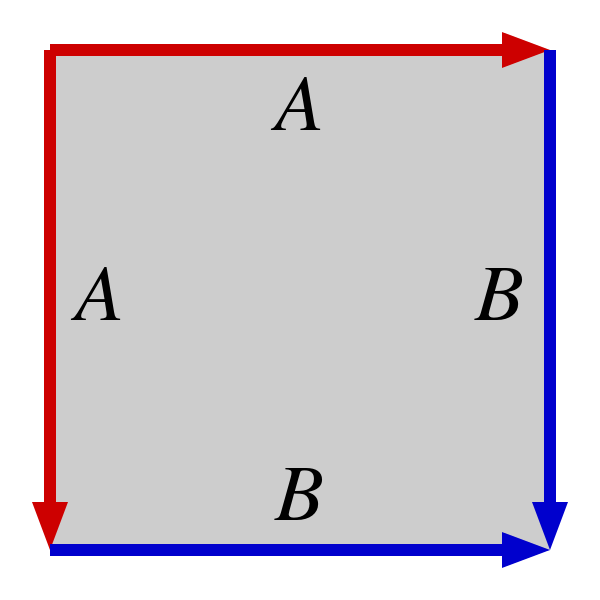
\includegraphics[scale = 0.1]{img/pol_fund_esfera}
		\end{figure}
		
		\item Podemos identificar el plano proyectivo real $\proy^2$ con un disco y una banda de Möbius donde la relación de equivalencia ``pega'' los bordes. También podemos identificarlo con una semiesfera en la que cada punto del borde es equivalente a su antípoda, o con una esfera completa en la que dos puntos están relacionados si y solo si son antipodales. Además, el polígono fundamental del plano proyectivo real sería:
		
		\begin{figure}[h!]
			\centering
			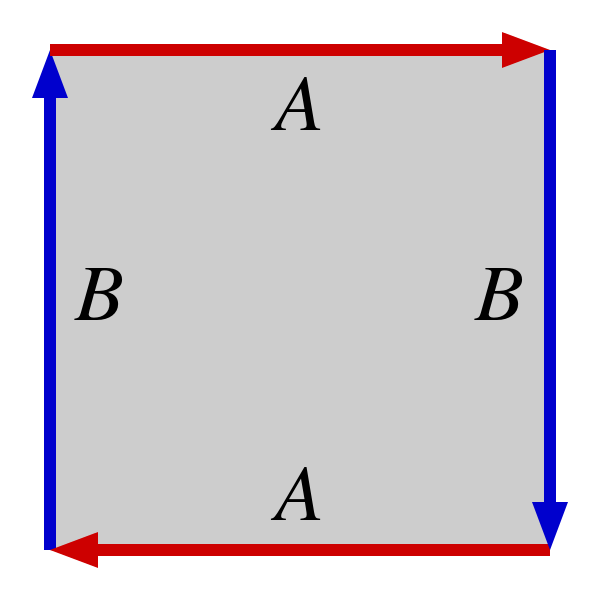
\includegraphics[scale = 0.1]{img/pol_fund_plano_proy}
		\end{figure}
		
		\item Vamos a ver otros dos polígonos fundamentales más. El de la banda de Möbius sería:
		
		\begin{figure}[h!]
			\centering
			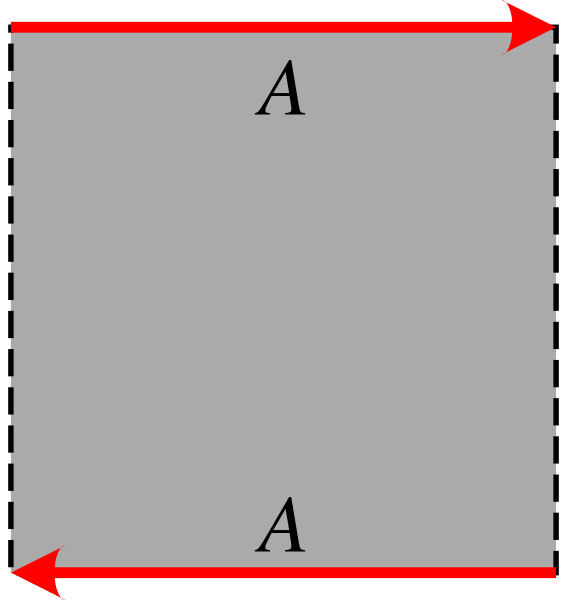
\includegraphics[scale = 0.09]{img/pol_fund_mobius}
		\end{figure}
		
		Nótese que en este caso hay un lado que no se pegaría, que corresponde al borde de la banda de Möbius. 
		\newpage
		Por otro lado, el de la botella de Klein sería:
		\begin{figure}[h!]
			\centering
			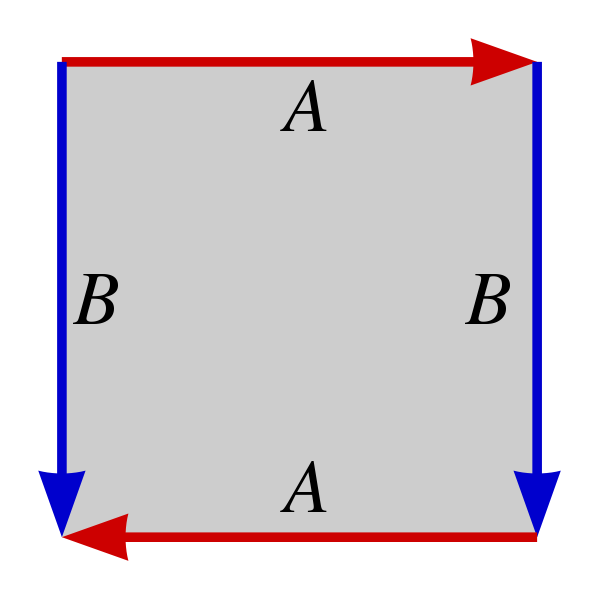
\includegraphics[scale = 0.1]{img/pol_fund_botella_klein}
		\end{figure}
	\end{enumerate}
\end{exa}

\section{Producto de espacios topológicos}
Una vez visto el caso del espacio cociente, pasamos ahora a realizar un desarrollo similar para otras construcciones como son los productos y sumas de espacios topológicos. Se va a realizar un procedimiento análogo en el desarrollo de las mismas al de la anterior sección.

Sean $(X_{i },\T_{i})^{1\le i\le r}$ espacios topológicos y sea $Y=\prod_i X_i$. Tomamos entonces 
\begin{equation}
Y=\prod_i X_i \stackrel{p_i^r}{\longrightarrow}(X_i,\T_i)
\end{equation}
Lo que buscamos en la construcción del espacio producto es dotar a $Y$ de la topología $\T$ más fina que haga continuas todas las aplicaciones $p_i^r$ para $1\le i\le r$. A dichas  $p_i^r$ las conoceremos a partir de ahora como \tbi[proyeccion@proyección]{proyecciones}.

De este modo, como queremos que $p_i^r$ sea continua  tenemos que para todo abierto $U_i\in \T_i$ deberá verificarse que $(p_i^r)^{-1}(U_i)=X_1\times\cdots\times U_i\times\cdots X_r$ (todos son los totales excepto en el caso de $X_i$) sea abierto. Es decir, que se cumpla $X_1\times\cdots\times U_i \times\cdots X_r\in \T$

Por lo tanto, vemos que por ser topología ha de verificarse que $(p_i^r)^{-1}(U_i)\cap (p_j^r)^{-1}(U_j)= X_1\cdots\times U_i \times\cdots\times U_j\times \cdots X_r$ sea parte de ella (intersección de abiertos).

Si tomamos ahora $ \{ U_1\times\cdots\times U_r : U_i\in \T_i \}$ veamos que es una base de la topología que pretendemos construir. Esto va a resultar evidente, ya que tan solo debemos comprobar para demostrarlo que al intersecar dos elementos cualesquiera de la base nos queda otro elemento de la base. 

Como dados $U_1\times\cdots\times U_r$ y $V_1\times\cdots\times V_r$ elementos de la base su intersección es $(U_1\cap V_1)\times\cdots\times (U_r\cap V_r)$ y como $(U_i\cap V_i)\in \T_i$, afirmamos que forma parte de la base por la definición de la misma.

Así, una vez que tenemos la base que va a caracterizar nuestra topología producto podemos afirmar que esta viene dada por $\T=\prod_i \T_i$.

\begin{defi}[Topología producto]
	Sean $(X_{i },\T_{i})^{1\le i\le r}$ espacios topológicos y sea $Y=\prod_i X_i$. Entonces se conoce como \tbitop[$\T_1\times\T_2$]{producto} a la topología $\T$ de $Y$ que viene dada por la base $ \{ U_1\times\cdots\times U_r : U_i\in \T_i \}$ (es decir, el producto de las topologías).
\end{defi}

Podemos formular, además, una propiedad universal del producto que caracteriza a esta topología:

\begin{lem}[Propiedad universal del producto]
	En la siguiente situación,
	\[\xymatrix{
		Y=\prod_i X_i \ar[r]^{p_i} & 
		(X_i,\T_i) \\
		(Z,\T') \ar[u]^{(f_1,\dots,f_n)=f} \ar[ru]_{p_i\circ f=f_i} &
	}\]
	tenemos la \tbi[propiedad universal!del producto]{propiedad universal del producto} que caracteriza la continuidad de $f$, diciendo que esta será continua si y solo si $f_i=p_i^r\circ f$ son continuas para todo $i$.
	
	\begin{proof}
		Vemos que si $f$ es continua, como $p_i^r$ son continuas, tenemos que $f_i$ también lo será al ser composición de estas.
		
		Por otro lado, tenemos que dado $W=\prod_iU_i$ abierto en $X$, tenemos que $f^{-1}(W)=\bigcap_i f_i^{-1}(U_i)$ será abierto dado que los $f_i^{-1}(U_i)$ son abiertos por ser $f$ continua. Así, como hemos probado que la imagen inversa de abiertos es abierta, tenemos que $f$ es continua.
	\end{proof}
\end{lem}

Veamos ahora que la propiedad universal caracteriza la topología.

\begin{prop}
	Si $(Y,\T_Y)$ cumple la propiedad universal del producto, entonces $\T_Y = \prod\T_i $
\end{prop}
\begin{proof}
	Vamos a demostrarlo por doble contención y haciendo algún cambalache con la identidad.
	Empecemos con un diagrama para aclarar las ideas.
	\[\xymatrix{
		(Y,\T_Y) \ar[r]_{p_{r_i}}^{p_i} & 
		(X_i,\T_i) \\
		(Y,\T_Y) \ar[u]^{\text{id}} \ar[ru]_{p_{r_i} = p_{r_i} \circ \text{ id}} &
	}\]
	Como la topología $\T_Y$ cumple la propiedad universal y la aplicación identidad es continua, tenemos que $p_{r_i}$ es continua. Luego por finura $ \prod\T_i \subset \T_Y$.
	
	Ahora razonamos con este diagrama:
	\[\xymatrix{
		(Y,\T_Y) \ar[r]_{p_{r_i}}^{p_i} & 
		(X_i,\T_i) \\
		(Y,\prod\T_i) \ar[u]^{\text{id}} \ar[ru]_{p_{r_i} = p_{r_i} \circ \text{ id}} &
	}\]	
	Como por construcción $p_{r_i}$ es continua, entones id es continua. Esto solo ocurre si $\T_Y \subset \prod\T_i$. 	
\end{proof}

Vamos a ver ahora una serie de proposiciones relacionadas con la topología producto, las cuales a pesar de resultar sencillas de comprobar nos proporcionan resultados interesantes.

\begin{prop}
	Las proyecciones son abiertas.
	
	\begin{proof}
		Sea $W$ abierto en el espacio producto, veamos que $p_i^r(W)$ es abierto.
		
		Nos basta con comprobarlo con los abiertos de la base, es decir, para los elementos de la forma $ U_1\times\cdots\times U_r : U_i\in \T_i$.  Como  $p_i^r(U_1\times\cdots\times U_r)=U_i$ es abierto podemos concluir la demostración.
	\end{proof}
\end{prop}


\begin{prop}
	La aplicación $f : X_i\to\{a_1\}\times\cdots\times X_i\times\cdots\times \{a_r\}\subset X_1\times\cdots\times X_r$ tal que $x\mapsto (a_1,\dots,x,\dots,a_r)$ es una inmersión.
	
	\begin{proof}
		Evidentemente, f es biyectiva. Por otra parte, $f$ es la aplicación $(k_1,\dots,id,\dots,k_r)$ continua, por serlo la identidad.
		Además, $f^{-1} = p_{r_i}\restriction_{\{a_1\}\times\dots\times X_i \times \dots \times\{a_r\}}$ es continua por serlo las proyecciones. Luego f es homeomorfismo.
	\end{proof}
\end{prop}

\begin{obs}[Consecuencias]
	La topología de $\{a_1\}\times\dots\times X_i \times \dots \times\{a_r\}$ es exactamente la de $X_i$. Esto constituye un truco para comprobar si una topología es una topología producto.
\end{obs}
	

Ahora pasamos a ver si somos capaces de construir bases más sencillas para nuestra topología producto, es decir, conformadas por menos abiertos. Igualmente, veremos el modo de construcción de bases de entornos en el espacio producto. No vamos a probar que sean bases realmente en ninguno de los dos casos ya que en ambos casos va a resultar muy sencillo aplicando la caracterización de base, dejándose como ejercicio para el lector de cara al repaso de la misma.
\begin{enumerate}
	\item Dado el espacio producto $(\prod_iX_i,\prod_i\T_i)$ tenemos que: \[\B=\{W_i\times\cdots\times W_r:W_i\in \B_i \text{ base de }\T_i\}\] es base de entornos del mismo.
	\begin{proof}
		Sea $\U \in \T$. Podemos descomponerlo como sigue $\U =U_1 \times \dots \times U_r $ con $U_i \in \T_i$ y $U_i = \bigcup_j W_{ij}$ con $W_{ij} \in \B_i$. Sea $x \in \U$. Entonces $x \in \W_{1j} \times \dots \times W_{rj} \subset \bigcup_j W_{1j} \times \dots \times \bigcup_j W_{rj} = U_1 \times \dots \times U_r$. Haciendo este procedimiento para cada punto se sigue el resultado.
	\end{proof}

	\item Dado el espacio producto $(\prod_iX_i,\prod_i\T_i)$ y $(a_1,\dots,a_r)\in\prod_iX_i$ tenemos que: \[\V_{(a_1,\dots,a_r)}=\{V_{a_1}\times\cdots\times V_{a_r}:W_i\in \V_{a_i} \text{ base de entornos en } \T_i\} \] es base de entornos del mismo.
\end{enumerate}

Por último, algunas observaciones útiles sobre la topología de los productos son
\begin{prop}[Adherencia]
	Sean $X_i$ espacios topológicos y $A_i$ subconjuntos de $X_i$. Tenemos que
	\[Adh(A_1 \times \dots \times A_r) = Adh(A_1) \times \dots \times Adh(A_r)\]
\end{prop}
\begin{proof}
	 Por una parte tenemos que $x \in Adh(A_1 \times \dots \times A_r) \iff$ dado un entorno $U_1 \times \dots \times U_r$ de $x$, dicho entorno corta a $A_1 \times \dots \times A_r$.
	 Por otra parte, $x \in  Adh(A_1) \times \dots \times Adh(A_r) \iff \ \forall U_1 \times \dots \times U_r $ se cumple que $U_i \cap A_i \neq \emptyset \ \forall i$.
	 Finalmente, gracias a la siguiente propiedad $(U_1 \times \dots \times U_r) \cap (A_1 \times \dots \times A_r) = (U_1 \cap A_1) \times \dots \times (U_r \cap A_r)$ se llega al resultado.
\end{proof}

\begin{prop}[Cerrados]
	Sean $X_i$ espacios topológicos y $A_i$ subconjuntos de $X_i$. Tenemos que
	$A_1 \times \dots \times A_r$ es cerrado $\iff A_i$ es cerrado $\forall i$.
\end{prop}
\begin{proof}
	Veamos que si $A_i$ es cerrado $\forall i$ entonces $A_1 \times \dots \times A_r$ es cerrado. Basta ver que $A_1 \times \dots \times A_r$ coincide con su adherencia, que por la proposición anterior coincide con $Adh(A_1) \times \dots \times Adh(A_r)$, que a su vez es $A_1 \times \dots \times A_r$, pues cada $A_i$ coincide con su adherencia por ser cerrado.
	La otra implicación se deja al lector.
\end{proof}	

		
\section{Suma}
Vamos a ver como última la construcción la suma, la cual gracias al desarrollo previo de los casos anteriores va a resultar de fácil comprensión para el lector. La idea de esta construcción va a ser la de realizar copias de objetos a distintas ``alturas'' (como si los colocáramos en estantes). 

Como antes, vamos a comenzar viendo las propiedades que debe cumplir la topología que caracterice nuestro espacio para luego pasar a construirla.

Dados los espacios $(X_i, \T_i)^{1\le i \le r}$ con sus correspondientes topologías, construimos el espacio suma como
\begin{equation}
(X_i, \T_i)\stackrel{j_i}\longrightarrow Y=\sum_{i=1}^rX_i=\bigcup_{i=1}^r\{i\}\times X_i
\end{equation}
Conviene resaltar que, como podemos observar, las copias de los distintos espacios $X_i$ en la suma será distinta, dado que a cada una le corresponderá un elemento $i$ distinto.

Ahora bien, nuestro objetivo en esta construcción será el de crear la topología $\T$ más fina en $Y$ de modo que haga las $j_i$ continuas. Las funciones $j_i$ las llamaremos \tbi{inclusiones}.

Por definición de continuidad, podemos (y debemos, ya que buscamos que sea la más fina) incluir en $\T$ todos los conjuntos de $Y$ cuya inversa sea abierta.
De este modo, también incluiremos $\{i\}\times X_i$ dado que $j^{-1}(\{i\}\times X_i)=X_i$ que es abierto en $\T_i$.

Ahora construimos la topología que tiene como base $\B=\{\{i\}\times U_i:U_i\in\T_i\}$ comprobemos que está bien definida y que es realmente base.
\begin{equation}
(\{i\}\times U_i)\cap(\{j\}\times U_j)=
\left\{ \begin{array}{lcc}
\{i\}\times(U_i\cap U_j)\in\T &   si  & i=j \\
\\  \emptyset\in\T& si & i\neq j 
\end{array}
\right.
\end{equation}
Como podemos ver, ambos casos verifican que la intersección está contenida en $\T$ como debiamos demostrar para ver que es base del mismo.
Así, podemos definir:
\begin{defi}[Topología suma]
	Dados los espacios con sus correspondientes topologías $(X_i, \T_i)^{1\le i \le r}$ y el espacio suma $Y=\sum_{i=1}^rX_i$, construimos la \tbitop{suma} como aquella topología que tiene como base $\B=\{\{i\}\times U_i:U_i\in\T_i\}$.
\end{defi}

Una vez vista su definición, veamos ahora un resultado fundamental acerca de la topología suma que no va a ser otra que la siguiente propiedad universal:

\begin{lem}[Propiedad universal de la suma]
	En la siguiente situación:
	\[\xymatrix{
		X \ar[rd]^f & \\
		X_i \ar[u]^{j_i} \ar[r]_{f_i} &
		Y
	}\]
	tomando en $X_i$ las topologías $\T_i$ y siendo $(Y,\T)$, tenemos la siguiente \tbi[propiedad universal!de la suma]{propiedad universal de la suma} que caracteriza la continuidad de $f$, diciendo que esta será continua si y solo si  $f_i=j_i\circ f$ son continuas para todo $i$.
	
	\begin{proof}
		Vemos que si $f$ es continua, como $j_i$ son continuas, tenemos que $f_i$ también lo será al ser composición de estas.
		
		Por otro lado, tenemos que dado que $(Y,\T)$ como hemos visto en la construcción de la topología suma $T$ es un recubrimiento abierto y continuo en cada uno de los $X_i$, tenemos que al ser continuo cada $f_i$ en $X_i$ también lo será $f$.
	\end{proof}
\end{lem}

Resulta importante indicar que como se desprende de la demostración (segunda implicación) la propiedad universal no solo nos va a caracterizar la función $g$, sino que nos permite caracterizar también la topología suma (si no se cumple la propiedad podemos asegurar que no estamos trabajando en esta). 

\begin{obs}
	Veamos por último un par de observaciones sobre esta topología que pueden resultar interesantes de cara a conocer el mecanismo de la misma.
	\begin{enumerate}
	\item Como hemos visto, $\{i\}\times X_i\subset\sum_j X_j$ siendo $\{i\}\times X_i$ abierto. Veamos que también es cerrado.
	
	Dado que $\sum_j X_j\setminus \{i\}\times X_i=\bigcup_{j\ne i }X_j$ es abierto, lo tenemos.
	
	\item Las inclusiones $X_l\stackrel{j_l}\longrightarrow\sum_iX_i$ son inmersiones abiertas y cerradas. Esto lo dejamos como ejercicio al lector, es un ejercicio sencillo pero puede resultar útil como repaso del modo de construcción de la topología suma realizado previamente en el apartado. \qedhere
\end{enumerate}
\end{obs}
